\section{Evaluation}
\label{sec:evaluation}

To measure the obtained C2 system maneuver agility, we assessed the proposed model under different scenarios based on the definition of the capacity to deal with dynamic circumstances by changing the C2 approach according to some criteria. This assessment is performed through an \textit{in silico} experiment~\cite{simulation01} simulating our motivating example (Section \ref{sec:motivation}). Such method provides a way to analyse different situations and it allows to work with different scenarios that would otherwise be unfeasible to test given incurred cost and resources availability. The simulated environment considers that the circumstances can change during the mission execution, allowing to test the effectiveness of the C2 System under such conditions.
 
%%%%%%%%%%%%%%%%%%%%%%%%%%%%%%%%%%
% SUBSECTION 
%%%%%%%%%%%%%%%%%%%%%%%%%%%%%%%%%%
\subsection{Definition}
\label{ssec:definition}

Our performed empirical study is defined according to the Goal-Question-Metric(GQM)~\citep{baier} method. Using this method, our purpose is to assess C2 maneuver agility from the C2 computational proposed model from the viewpoint of a researcher in the context of a software Simulation of UAV's employment in a reconnaissance mission. From the goal, our research question is \textit{How much C2 maneuver agility the system has?}. 

Next, we define the metrics applied in the evaluation to answer the proposed question and their corresponding descriptions:
\begin{itemize}
    \item Maneuvering (M1): Number of C2 Maneuvers performed by the members to accomplish the mission within a given timeout;
    \item Timeliness (M2): System time, in ticks, to accomplish the mission within a given timeout;
    \item Effectiveness (M3): Percentage of successful tasks completed by the executors.
\end{itemize}

To measure agility, three metrics are applied (\textit{M1 - Maneuvering; M2 - Timeliness; M3 - Effectiveness}). Context perturbations, i.e., onboard component damage or sudden changes in the environment, require system adaptation to keep running. In such conditions, the number of C2 Approach changes are counted, i.e., M1 (Maneuvering), to identify their adaptability level of the system due to its capability of changing its organization.

All reconfigurations in the C2 approach and tasks execution, must take place in a timely manner. Such response time is measured by the M2 (Timeliness) metric, i.e., timeliness, which marks how long the system has acted to execute mission's tasks. This highlights the responsiveness of the system to changing circumstances. Furthermore, the ration of mission's tasks that has already been accomplished by the elements in view of the dynamic context is evaluated, i.e., M3 (Effectiveness) metric.

%%%%%%%%%%%%%%%%%%%%%%%%%%%%%%%%%%
% SUBSECTION 
%%%%%%%%%%%%%%%%%%%%%%%%%%%%%%%%%%
\subsection{Planning}
\label{ssec:planning}

The following subsections describe the considered hypotheses to validate the proposed model (Subsection~\ref{sssec:hyp}), define the elements that compose the scenarios (Subsection~\ref{sssec:scenarios}), and explain the experimental design to run the considered scenarios (Subsection~\ref{sssec:design}).

\subsubsection{Hypothesis Formulation}
\label{sssec:hyp}

Figure~\ref{fig:variables} shows the factors and the dependent variables that represent the results in our GQM. The scenario and the action method are identified as factors. A scenario comprises an initial context and a sequence of events that occur during the mission. Section~\ref{sssec:scenarios} details possible scenarios.

\begin{figure}[ht!]
    \centering
    \scalebox{.65}{

\tikzset{every picture/.style={line width=0.75pt}} %set default line width to 0.75pt        

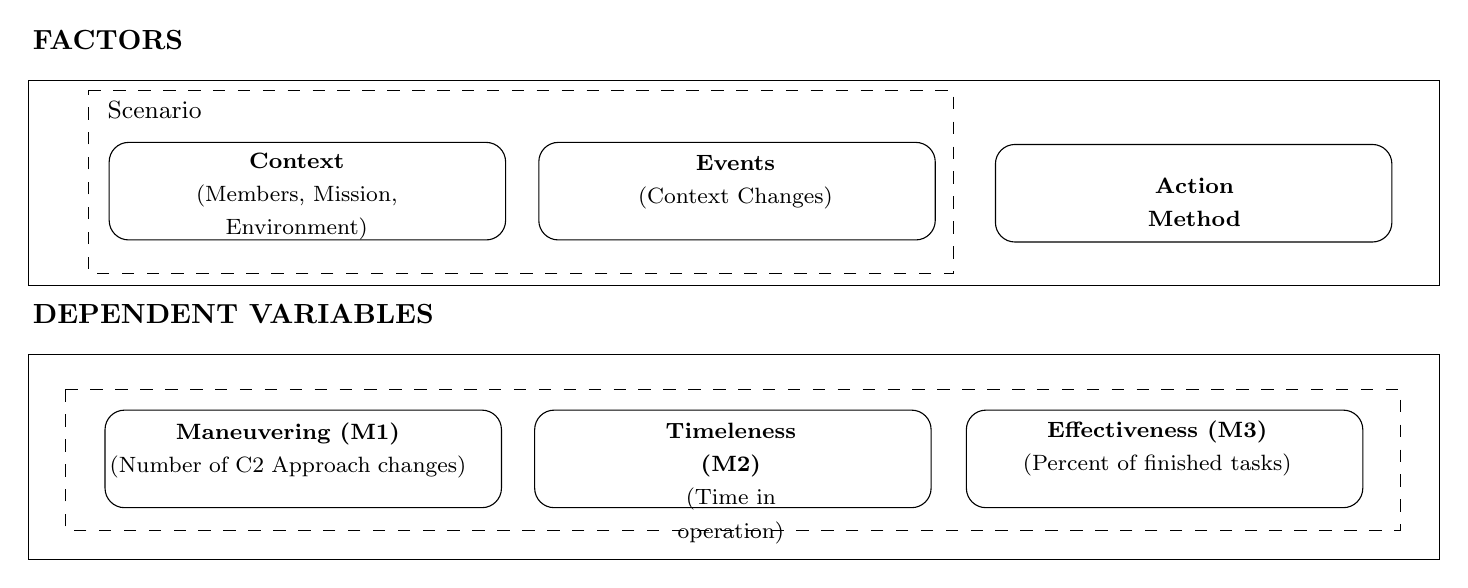
\begin{tikzpicture}[x=0.75pt,y=0.75pt,yscale=-1,xscale=1]
%uncomment if require: \path (0,511); %set diagram left start at 0, and has height of 511

%Shape: Rectangle [id:dp2552012932916572] 
\draw  [color={rgb, 255:red, 0; green, 0; blue, 0 }  ,draw opacity=1 ] (11,101) -- (691,101) -- (691,200) -- (11,200) -- cycle ;
%Rounded Rect [id:dp9161828495455207] 
\draw   (50,140.4) .. controls (50,135.21) and (54.21,131) .. (59.4,131) -- (231.6,131) .. controls (236.79,131) and (241,135.21) .. (241,140.4) -- (241,168.6) .. controls (241,173.79) and (236.79,178) .. (231.6,178) -- (59.4,178) .. controls (54.21,178) and (50,173.79) .. (50,168.6) -- cycle ;
%Rounded Rect [id:dp47914804412585] 
\draw   (257,140.4) .. controls (257,135.21) and (261.21,131) .. (266.4,131) -- (438.6,131) .. controls (443.79,131) and (448,135.21) .. (448,140.4) -- (448,168.6) .. controls (448,173.79) and (443.79,178) .. (438.6,178) -- (266.4,178) .. controls (261.21,178) and (257,173.79) .. (257,168.6) -- cycle ;
%Rounded Rect [id:dp36207445324802223] 
\draw   (477,141.4) .. controls (477,136.21) and (481.21,132) .. (486.4,132) -- (658.6,132) .. controls (663.79,132) and (668,136.21) .. (668,141.4) -- (668,169.6) .. controls (668,174.79) and (663.79,179) .. (658.6,179) -- (486.4,179) .. controls (481.21,179) and (477,174.79) .. (477,169.6) -- cycle ;
%Shape: Rectangle [id:dp7958558916033278] 
\draw  [dash pattern={on 4.5pt off 4.5pt}] (40,106) -- (457,106) -- (457,194) -- (40,194) -- cycle ;
%Shape: Rectangle [id:dp34078076660428835] 
\draw  [color={rgb, 255:red, 0; green, 0; blue, 0 }  ,draw opacity=1 ] (11,233) -- (691,233) -- (691,332) -- (11,332) -- cycle ;
%Rounded Rect [id:dp614914351003329] 
\draw   (48,269.4) .. controls (48,264.21) and (52.21,260) .. (57.4,260) -- (229.6,260) .. controls (234.79,260) and (239,264.21) .. (239,269.4) -- (239,297.6) .. controls (239,302.79) and (234.79,307) .. (229.6,307) -- (57.4,307) .. controls (52.21,307) and (48,302.79) .. (48,297.6) -- cycle ;
%Rounded Rect [id:dp9126417804308116] 
\draw   (255,269.4) .. controls (255,264.21) and (259.21,260) .. (264.4,260) -- (436.6,260) .. controls (441.79,260) and (446,264.21) .. (446,269.4) -- (446,297.6) .. controls (446,302.79) and (441.79,307) .. (436.6,307) -- (264.4,307) .. controls (259.21,307) and (255,302.79) .. (255,297.6) -- cycle ;
%Shape: Rectangle [id:dp68280710046261] 
\draw  [dash pattern={on 4.5pt off 4.5pt}] (29,250) -- (672,250) -- (672,318) -- (29,318) -- cycle ;
%Rounded Rect [id:dp2824039190738554] 
\draw   (463,269.4) .. controls (463,264.21) and (467.21,260) .. (472.4,260) -- (644.6,260) .. controls (649.79,260) and (654,264.21) .. (654,269.4) -- (654,297.6) .. controls (654,302.79) and (649.79,307) .. (644.6,307) -- (472.4,307) .. controls (467.21,307) and (463,302.79) .. (463,297.6) -- cycle ;

% Text Node
\draw (12,76) node [anchor=north west][inner sep=0.75pt]   [align=left] {\textbf{FACTORS}};
% Text Node
\draw (56,135) node [anchor=north west][inner sep=0.75pt]   [align=left] {\begin{minipage}[lt]{124.70588000000001pt}\setlength\topsep{0pt}
\begin{center}
\textbf{{\footnotesize Context}}\\{\footnotesize (Members, Mission, Environment)}
\end{center}

\end{minipage}};
% Text Node
\draw (303,136) node [anchor=north west][inner sep=0.75pt]   [align=left] {\begin{minipage}[lt]{71.20892pt}\setlength\topsep{0pt}
\begin{center}
{\footnotesize \textbf{Events}}\\{\footnotesize (Context Changes)}
\end{center}

\end{minipage}};
% Text Node
\draw (532,147) node [anchor=north west][inner sep=0.75pt]   [align=left] {\begin{minipage}[lt]{59.38310800000001pt}\setlength\topsep{0pt}
\begin{center}
{\footnotesize \textbf{Action Method}}
\end{center}

\end{minipage}};
% Text Node
\draw (48,110) node [anchor=north west][inner sep=0.75pt]   [align=left] {{\small Scenario}};
% Text Node
\draw (12,208) node [anchor=north west][inner sep=0.75pt]   [align=left] {\textbf{DEPENDENT VARIABLES}};
% Text Node
\draw (49,265) node [anchor=north west][inner sep=0.75pt]   [align=left] {\begin{minipage}[lt]{128.81784pt}\setlength\topsep{0pt}
\begin{center}
{\footnotesize \textbf{Maneuvering (M1)}}\\{\footnotesize (Number of C2 Approach changes)}
\end{center}

\end{minipage}};
% Text Node
\draw (301,265) node [anchor=north west][inner sep=0.75pt]   [align=left] {\begin{minipage}[lt]{70.90088000000002pt}\setlength\topsep{0pt}
\begin{center}
{\footnotesize \textbf{Timeleness (M2)}}\\{\footnotesize (Time in operation)}
\end{center}

\end{minipage}};
% Text Node
\draw (489,264) node [anchor=north west][inner sep=0.75pt]   [align=left] {\begin{minipage}[lt]{97.05912000000001pt}\setlength\topsep{0pt}
\begin{center}
{\footnotesize \textbf{Effectiveness (M3)}}\\{\footnotesize (Percent of finished tasks)}
\end{center}

\end{minipage}};


\end{tikzpicture}}
    \caption{Factors and dependent variables used by the proposed model}
    \label{fig:variables}
\end{figure}

The second factor is called action method and it represents how the system response is in order to solve a circumstance change or perturbation. With two possible values, i.e., A1 and A2, that identifies the baseline and the proposal in order to respond context changes, respectively. With A1 method, the system starts the execution with an initial context predefined and it performs a task allocation, i.e., distributing the mission received, and in face of context changes, e.g., member dropped, the system keeps running, but it does not perform any kind of adaptation to deal with new circumstances. In its turn, the A2 method applies the C2 computational design proposed in Section~\ref{sec:channelSystem} and whose implementation is described in Section~\ref{sec:design}. 

Considering the research questions and the metrics identified in GQM, it is possible to formulate the corresponding null and alternative hypotheses as shown:

$$H_0\: : \:\forall m \in Metric, \forall s \in Scenario \bullet (m(s \times A1)=m(s \times A2)$$

$$H_1\: : \:\forall m \in Metric, \forall s \in Scenario \bullet (m(s \times A1) \neq m(s \times A2)$$

The null hypotheses states no differences in metrics' average for different action methods in the same scenario. In contrast, the alternative hypotheses states otherwise. In $H_1$, for all metrics in GQM, i.e., M1, M2, and M3, different results for two different treatments are collected, i.e., A1 and A2, applied to the factor agility method. This difference in results can confirm the presence of C2 maneuver agility and its impact on the system.

%%%%%%%%%%%%%%%%%%%%%%%%%%%%%%%%%%
% SUBSECTION 
%%%%%%%%%%%%%%%%%%%%%%%%%%%%%%%%%%
\subsubsection{Simulation Scenarios}
\label{sssec:scenarios}

A simulation scenario is composed of an initial context and a sequence of events that provide dynamism. The initial context comprises the set $E$ of members operating an initial C2 Approach $\omega$, the mission $M$ composed of a set of tasks, and the environment. Each event in the set $CtxAct$ (Equation~\ref{eq:ctxact}) represents an action that causes a member or environment changes in runtime. Figure~\ref{fig:scenario} shows scenario's composition.

\begin{equation}
    \label{eq:ctxact}
    CtxAct = \{memberFailure,sensorFailure, envChange \} 
\end{equation}

The environment represents all the conditions of the place where the members act, e.g., weather conditions, hazard, and communication restrictions, and it is modelled as the state of a specific kind of onboard sensor, i.e., a foggy day can turn a VGA sensor useless.

\begin{figure}[ht!]
    \centering
    \scalebox{.6}{

\tikzset{every picture/.style={line width=0.75pt}} %set default line width to 0.75pt        

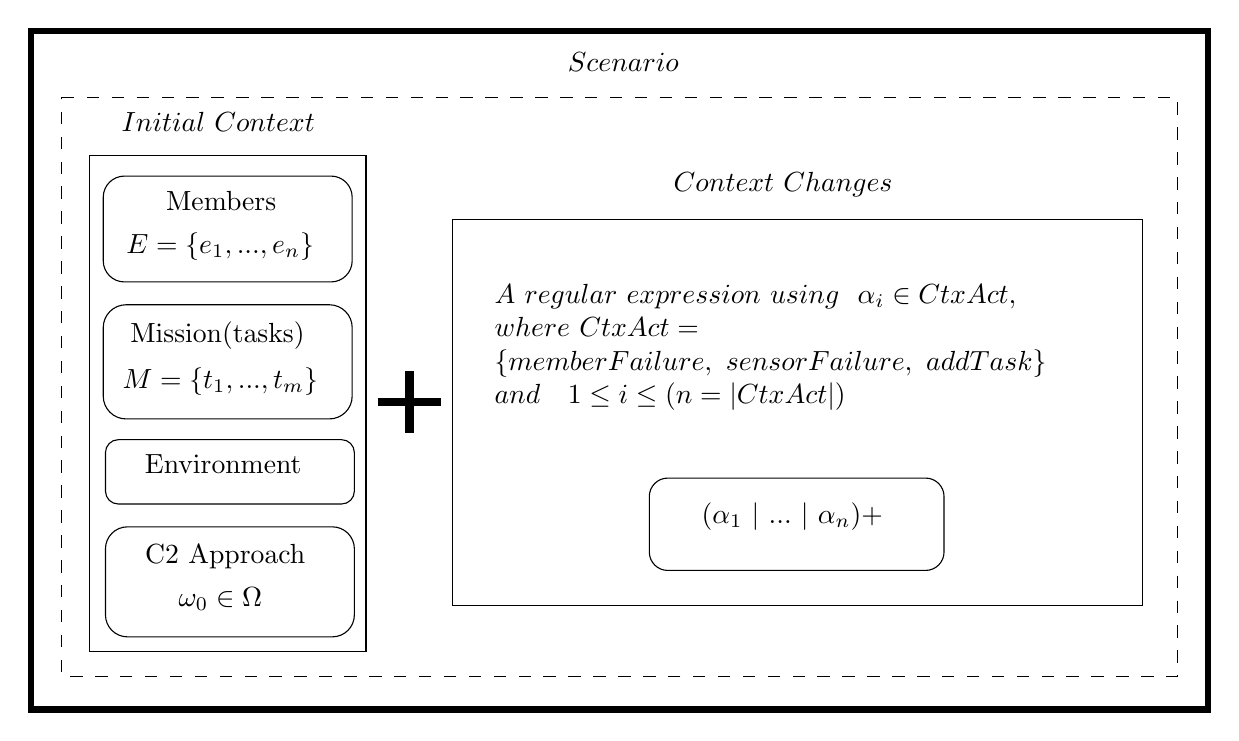
\begin{tikzpicture}[x=0.75pt,y=0.75pt,yscale=-1,xscale=1]
%uncomment if require: \path (0,354); %set diagram left start at 0, and has height of 354

%Rounded Rect [id:dp4190516071959901] 
\draw   (45.48,212.2) .. controls (45.48,208.78) and (48.25,206) .. (51.68,206) -- (159.2,206) .. controls (162.63,206) and (165.4,208.78) .. (165.4,212.2) -- (165.4,230.8) .. controls (165.4,234.22) and (162.63,237) .. (159.2,237) -- (51.68,237) .. controls (48.25,237) and (45.48,234.22) .. (45.48,230.8) -- cycle ;
%Rounded Rect [id:dp916271795400267] 
\draw   (44.41,152) .. controls (44.41,145.92) and (49.34,141) .. (55.41,141) -- (153.34,141) .. controls (159.41,141) and (164.34,145.92) .. (164.34,152) -- (164.34,185) .. controls (164.34,191.08) and (159.41,196) .. (153.34,196) -- (55.41,196) .. controls (49.34,196) and (44.41,191.08) .. (44.41,185) -- cycle ;
%Rounded Rect [id:dp6771464113681669] 
\draw   (44.41,89.2) .. controls (44.41,83.57) and (48.98,79) .. (54.61,79) -- (154.14,79) .. controls (159.77,79) and (164.34,83.57) .. (164.34,89.2) -- (164.34,119.8) .. controls (164.34,125.43) and (159.77,130) .. (154.14,130) -- (54.61,130) .. controls (48.98,130) and (44.41,125.43) .. (44.41,119.8) -- cycle ;
%Shape: Rectangle [id:dp977819802873701] 
\draw   (37.75,69) -- (171,69) -- (171,308) -- (37.75,308) -- cycle ;
%Rounded Rect [id:dp11904903891609209] 
\draw   (45.48,258.6) .. controls (45.48,252.75) and (50.22,248) .. (56.08,248) -- (154.8,248) .. controls (160.66,248) and (165.4,252.75) .. (165.4,258.6) -- (165.4,290.4) .. controls (165.4,296.25) and (160.66,301) .. (154.8,301) -- (56.08,301) .. controls (50.22,301) and (45.48,296.25) .. (45.48,290.4) -- cycle ;

%Shape: Rectangle [id:dp6932811140385843] 
\draw  [dash pattern={on 4.5pt off 4.5pt}] (24.5,41) -- (562,41) -- (562,320) -- (24.5,320) -- cycle ;
%Shape: Rectangle [id:dp3952140034216508] 
\draw  [line width=2.25]  (9.5,9) -- (576.5,9) -- (576.5,336) -- (9.5,336) -- cycle ;
%Shape: Rectangle [id:dp32385330595430617] 
\draw   (212.5,100) -- (545,100) -- (545,286) -- (212.5,286) -- cycle ;
%Rounded Rect [id:dp6771891907604983] 
\draw   (307.5,233.4) .. controls (307.5,228.48) and (311.48,224.5) .. (316.4,224.5) -- (440.6,224.5) .. controls (445.52,224.5) and (449.5,228.48) .. (449.5,233.4) -- (449.5,260.1) .. controls (449.5,265.02) and (445.52,269) .. (440.6,269) -- (316.4,269) .. controls (311.48,269) and (307.5,265.02) .. (307.5,260.1) -- cycle ;

\draw  [line width=3]  (177,188) -- (207,188)(192,173) -- (192,203) ;

% Text Node
\draw (267,18) node [anchor=north west][inner sep=0.75pt]    {$Scenario$};
% Text Node
\draw (393,287) node [anchor=north west][inner sep=0.75pt]    {$\ \ $};
% Text Node
\draw (318,76) node [anchor=north west][inner sep=0.75pt]    {$Context\ Changes$};
% Text Node
\draw (52,47) node [anchor=north west][inner sep=0.75pt]    {$Initial\ Context$};
% Text Node
\draw (225,128) node [anchor=north west][inner sep=0.75pt]    {$ \begin{array}{l}
A\ regular\ expression\ using\ \ \alpha _{i} \in CtxAct,\ \\
where\ CtxAct=\\
\{memberFailure,\ sensorFailure,\ addTask\} \ \\
and\ \ \ 1\leq i\leq ( n=|CtxAct|)
\end{array}$};
% Text Node
\draw (327,235) node [anchor=north west][inner sep=0.75pt]    {$\ ( \alpha _{1} \ |\ ...\ |\ \alpha _{n}) +$};
% Text Node
\draw (73.42,85) node [anchor=north west][inner sep=0.75pt]   [align=left] {Members};
% Text Node
\draw (56.17,148) node [anchor=north west][inner sep=0.75pt]   [align=left] {Mission(tasks)};
% Text Node
\draw (63.24,212) node [anchor=north west][inner sep=0.75pt]   [align=left] {Environment};
% Text Node
\draw (54.32,105) node [anchor=north west][inner sep=0.75pt]    {$E=\{e_{1} ,...,e_{n}\}$};
% Text Node
\draw (52.42,170) node [anchor=north west][inner sep=0.75pt]    {$M=\{t_{1} ,...,t_{m}\}$};
% Text Node
\draw (63.37,255) node [anchor=north west][inner sep=0.75pt]   [align=left] {C2 Approach};
% Text Node
\draw (79.49,276) node [anchor=north west][inner sep=0.75pt]    {$\omega _{0} \in \Omega $};


\end{tikzpicture}}
    \caption{Scenario composed of the initial context variables and a sequence of events that characterizes a dynamic context}
    \label{fig:scenario}
\end{figure}

The possible actions combined with the initial context used by the simulation are listed in Table~\ref{table:context_changes}. These actions are called during simulation to create a dynamic scenario, resembling realistic settings. Despite the possible infinite number of scenarios, a subset of actions was selected to be simulated. The scenarios were created with different sequences of actions, i.e., context changes, combined with the same initial context, i.e., members, mission, environment and the initial C2 Approach. 

\begin{table}[ht]
	\small
	\fontsize{10}{10}\selectfont
	\centering
	\caption{Context changes handled by the simulator with related actions in the CS and their impact level in the system}
	\label{table:context_changes}
	
	\begin{tabular}{p{0.15\linewidth}p{0.15\linewidth}p{0.50\linewidth}}
	\hline
		 \textbf{Context Change}
		& \textbf{Action}
		& \textbf{Description}  \\ [2ex]
	\hline	
	Self & \textit{sensorFailure} & Sensor onboard damage caused by any internal issue (electronic circuit damaged) \\[1ex]
	& \textit{memberFailure} & UAV out of operation due to serious damage (e.g., no fuel or battery, or taken down) \\[5ex]
	
	%Mission & addTasks & 1 & tasks addition or removal in the mission \\[5ex]
	
	Environment & \textit{envChange} & Weather conditions (e.g., luminosity, cloudiness) impacting the sensor's quality; \\[1ex]
	& & Hazard level requiring changes in the UAV's behaviour \\[1ex]
	\hline
	\end{tabular}
\end{table} 


Table~\ref{tab:scenarios} shows all sequences of events used by the treatments of context change factor. In addition, the submission of such scenarios to the military domain experts~\citep{nato01, doctrine01, Fernandes2016, UAV_Aplication, CC03, UAV01} allowed the creation of sequences compatible with possible real conditions and that follow concrete analysis of complexity. During simulation, all these changes occur within the timeout, i.e., mission time limit, but not equally distributed over time. The presented sequence is attended but the exact moment is aleatory.

\begin{table}[h]
\centenring
\fontsize{9}{9}
\selectfont
\caption{List of events(\textit{EC-envChange; SF-sensorFailure; MF-memberFailure}) that characterizes the context changes within the scenarios tested. The initial C2 Approach, the set of members $E$ and the mission $M$ remain unchanged.}
\label{tab:scenarios}
\begin{tabular}{|m{0.1\textwidth}|m{0.84\textwidth}|}
\hline
\rowcolor{lightgray}
 \textbf {Scenario} & \hfil  \textbf {Context Changes} \\
\hline
 \hfil 1 & EC $\rightarrow$ EC $\rightarrow$ EC $\rightarrow$ EC $\rightarrow$ EC\\
\hline 
 \hfil 2 & EC $\rightarrow$ EC $\rightarrow$ EC $\rightarrow$ EC $\rightarrow$ EC $\rightarrow$ EC $\rightarrow$ EC $\rightarrow$ EC $\rightarrow$ EC $\rightarrow$ EC $\rightarrow$ EC $\rightarrow$ EC $\rightarrow$ EC $\rightarrow$ EC $\rightarrow$ EC \\
\hline 
 \hfil 3 & 
EC $\rightarrow$ EC $\rightarrow$ EC $\rightarrow$ EC $\rightarrow$ EC $\rightarrow$ MF $\rightarrow$ EC $\rightarrow$ EC $\rightarrow$ EC $\rightarrow$ EC $\rightarrow$ EC $\rightarrow$ MF $\rightarrow$ EC $\rightarrow$ EC $\rightarrow$ EC $\rightarrow$ EC $\rightarrow$ EC $\rightarrow$ MF $\rightarrow$ EC $\rightarrow$ EC $\rightarrow$ EC $\rightarrow$ EC $\rightarrow$ EC  \\
\hline 
 \hfil 4 & EC $\rightarrow$ EC $\rightarrow$ EC $\rightarrow$ EC $\rightarrow$ EC $\rightarrow$ SF $\rightarrow$ EC $\rightarrow$ EC $\rightarrow$ EC $\rightarrow$ EC $\rightarrow$ EC $\rightarrow$ SF $\rightarrow$ EC $\rightarrow$ EC $\rightarrow$ EC $\rightarrow$ EC $\rightarrow$ EC $\rightarrow$ SF $\rightarrow$ EC $\rightarrow$ EC $\rightarrow$ EC $\rightarrow$ EC $\rightarrow$ EC  \\
\hline 
 \hfil 5 & EC $\rightarrow$ EC $\rightarrow$ EC $\rightarrow$ SF $\rightarrow$ EC $\rightarrow$ EC $\rightarrow$ EC $\rightarrow$ MF $\rightarrow$ EC $\rightarrow$ EC $\rightarrow$ EC $\rightarrow$ SF $\rightarrow$ EC $\rightarrow$ EC $\rightarrow$ EC $\rightarrow$ MF $\rightarrow$ EC $\rightarrow$ EC $\rightarrow$ EC $\rightarrow$ SF $\rightarrow$ EC $\rightarrow$ EC $\rightarrow$ EC $\rightarrow$ MF  \\
\hline 
 \hfil 6 & EC $\rightarrow$ SF $\rightarrow$ MF $\rightarrow$ EC $\rightarrow$ SF $\rightarrow$ EC $\rightarrow$ SF $\rightarrow$ EC $\rightarrow$ SF $\rightarrow$ MF $\rightarrow$ EC $\rightarrow$ SF $\rightarrow$ EC $\rightarrow$ SF $\rightarrow$ EC $\rightarrow$ SF \\
\hline 
 \hfil 7 & MF $\rightarrow$ SF $\rightarrow$ EC $\rightarrow$ EC $\rightarrow$ EC $\rightarrow$ EC $\rightarrow$ EC $\rightarrow$ EC $\rightarrow$ EC $\rightarrow$ EC $\rightarrow$ EC $\rightarrow$ EC $\rightarrow$ MF $\rightarrow$ SF $\rightarrow$ EC $\rightarrow$ EC $\rightarrow$ EC $\rightarrow$ EC $\rightarrow$ EC $\rightarrow$ MF $\rightarrow$ SF $\rightarrow$ EC $\rightarrow$ EC $\rightarrow$ EC $\rightarrow$ MF $\rightarrow$ SF $\rightarrow$ EC \\
 \hline
 \hfil 8 & MF $\rightarrow$ SF $\rightarrow$ EC $\rightarrow$ MF $\rightarrow$ SF $\rightarrow$ EC $\rightarrow$ MF $\rightarrow$ SF $\rightarrow$ EC $\rightarrow$ MF $\rightarrow$ SF $\rightarrow$ EC \\
 \hline
 \hfil 9 & SF $\rightarrow$ SF $\rightarrow$ SF $\rightarrow$ MF $\rightarrow$ SF $\rightarrow$ SF $\rightarrow$ SF $\rightarrow$ MF $\rightarrow$ SF $\rightarrow$ SF $\rightarrow$ SF $\rightarrow$ MF $\rightarrow$ SF $\rightarrow$ SF $\rightarrow$ SF \\
 \hline
 \hfil 10 & SF $\rightarrow$ EC $\rightarrow$ MF $\rightarrow$ SF $\rightarrow$ EC $\rightarrow$ MF $\rightarrow$ SF $\rightarrow$ EC $\rightarrow$ MF $\rightarrow$ SF $\rightarrow$ EC $\rightarrow$ MF $\rightarrow$ EC $\rightarrow$ EC $\rightarrow$ EC $\rightarrow$ EC $\rightarrow$ EC $\rightarrow$ EC $\rightarrow$ EC $\rightarrow$ EC $\rightarrow$ EC $\rightarrow$ EC \\
 \hline
\end{tabular}

\end{table}


The simulation operates a scenario with 5 possible types of tasks (0 to 4) and 5 types of sensors (A, B, C, D and E) whereas only one random sensor per executor is active during the entire simulation. The tasks and sensors onboard are randomly chosen before the running round. When the tasks allocation process starts, the algorithm applies a function that returns the quality $Q_{ij}$, obtained from a table, that correlates a sensor $i$ to the task $j$. When $Q_{ij}=0$ it means the sensor $i$ is not able to perform the task $j$.

%%%%%%%%%%%%%%%%%%%%%%%%%%%%%%%%%%
% SUBSECTION 
%%%%%%%%%%%%%%%%%%%%%%%%%%%%%%%%%%
\subsubsection{Experimental Design}
\label{sssec:design}


Figure \ref{fig:exp_design} shows the experimental design applied to assess the formulated hypotheses. A factorial experiment is performed with the treatments applied to the simulation scenario (cf. Section~\ref{sssec:scenarios}) and to the action method. Combinations of the factors are assessed with the metrics described in Section~\ref{ssec:definition}.

\begin{figure}[ht!]
    \centering
    \scalebox{.65}{

\tikzset{every picture/.style={line width=0.75pt}} %set default line width to 0.75pt        

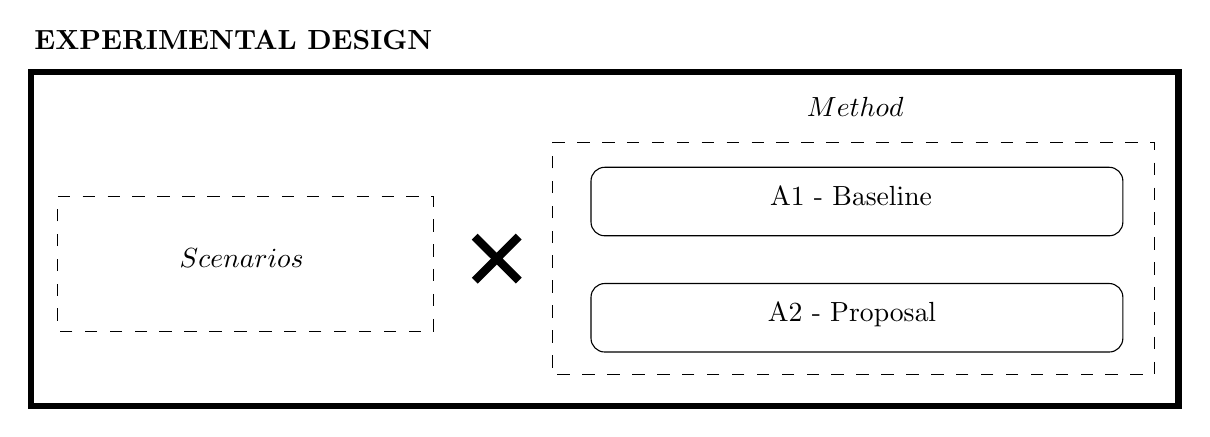
\begin{tikzpicture}[x=0.75pt,y=0.75pt,yscale=-1,xscale=1]
%uncomment if require: \path (0,201); %set diagram left start at 0, and has height of 201

%Rounded Rect [id:dp06575569211056953] 
\draw   (279.42,79.6) .. controls (279.42,75.95) and (282.37,73) .. (286.02,73) -- (529.06,73) .. controls (532.7,73) and (535.66,75.95) .. (535.66,79.6) -- (535.66,99.4) .. controls (535.66,103.05) and (532.7,106) .. (529.06,106) -- (286.02,106) .. controls (282.37,106) and (279.42,103.05) .. (279.42,99.4) -- cycle ;
%Shape: Rectangle [id:dp6932811140385843] 
\draw  [dash pattern={on 4.5pt off 4.5pt}] (22.5,87) -- (203.5,87) -- (203.5,152) -- (22.5,152) -- cycle ;
%Shape: Rectangle [id:dp9822494345299366] 
\draw  [dash pattern={on 4.5pt off 4.5pt}] (260.75,61) -- (551,61) -- (551,173) -- (260.75,173) -- cycle ;
%Shape: Rectangle [id:dp3952140034216508] 
\draw  [line width=2.25]  (9.5,27) -- (562.5,27) -- (562.5,188) -- (9.5,188) -- cycle ;
\draw  [line width=3]  (223.37,106.42) -- (244.63,127.58)(244.58,106.37) -- (223.42,127.63) ;
%Rounded Rect [id:dp9781270849297624] 
\draw   (279.42,135.6) .. controls (279.42,131.95) and (282.37,129) .. (286.02,129) -- (529.06,129) .. controls (532.7,129) and (535.66,131.95) .. (535.66,135.6) -- (535.66,155.4) .. controls (535.66,159.05) and (532.7,162) .. (529.06,162) -- (286.02,162) .. controls (282.37,162) and (279.42,159.05) .. (279.42,155.4) -- cycle ;

% Text Node
\draw (80,111) node [anchor=north west][inner sep=0.75pt]    {$Scenarios$};
% Text Node
\draw (382.17,38) node [anchor=north west][inner sep=0.75pt]    {$Method$};
% Text Node
\draw (10,6) node [anchor=north west][inner sep=0.75pt]   [align=left] {\textbf{EXPERIMENTAL DESIGN}};
% Text Node
\draw (364.41,81) node [anchor=north west][inner sep=0.75pt]   [align=left] {A1 - Baseline};
% Text Node
\draw (363.41,137) node [anchor=north west][inner sep=0.75pt]   [align=left] {A2 - Proposal};


\end{tikzpicture}}
    \caption{Experimental design with the treatments performed by the simulator}
    \label{fig:exp_design}
\end{figure}

The simulation uses a set of random variables to define some elements during execution, i.e., UAVs and tasks position, and sensor that will be affected by the context event. For a consistent comparison between the action methods A1 and A2, the same set of random variables is used by both methods during the same execution number. 

Furthermore, we insert in runtime some perturbations and factors modifications to provide dynamism to the system and become it closer to a real scenario. A context change simulated by the system causes the quality reducing of a specific type of sensor, e.g., an environment change simulating a luminosity decreasing reduces in $50\%$ the quality of the sensor type 2 that represents a VGA camera. in case of the sensor burns out, its quality comes to be zero and the task will be transmitted to another member to check its execution capacity. Furthermore, we can lose a member and, consequently, all its sensors onboard.

Context changes can generate situations such the tasks reallocation is not enough to keep mission execution. In that case, the C2 System performs a C2 Approach change, i.e., a maneuvering. The new C2 Approach operated can provide a higher awareness level, i.e., more information shared by the members with a new communication structure, and it can help the members perform reallocation based on the new data exchanged. The initial C2 Approach for all scenarios simulated is De-Conflicted, i.e., a ring communication structure. From this C2 Approach, the maneuver follows incrementally over a specific order of C2 approaches, based on the following research~\cite{france2014}, and going back to Conflicted after Edge. The Conflicted is the final C2 Approach adopted by the system before discarding the unfeasible tasks.


%%%%%%%%%%%%%%%%%%%%%%%%%%%%%%%%%%
% SUBSECTION 
%%%%%%%%%%%%%%%%%%%%%%%%%%%%%%%%%%
\subsection{Executions}
\label{subsec:operations}

The experiment performs a set of executions in batch way to reduce the standard deviation in results obtained. An initial number of runs ($n_i=50$) was chosen to analyse the amount of dispersion in the results obtained by the experiments. Based on this, it was demonstrated the need to adjust the sample size in order to meet an acceptable confidence level. According to \cite{CochranW.G.1983}, Equation~\ref{eq:stat} gives the sample size that satisfies a given confidence level, a population standard deviation $\sigma$, and a difference($d$) between the population mean($\overline{X}$) and sample mean($\mu$).

\begin{equation}
    \label{eq:stat}
    n=\left(\frac{Z_{\alpha/2} \cdot \sigma}{d}\right)^2
\end{equation}

Equation~\ref{eq:stat} is applied with $95\%$ confidence, i.e., a $Z_{\alpha/2} = 1.96$, and $d = |\overline{X} - \mu| \leq .1\mu_i$, where $\mu_i$ is the mean obtained with the initial set of runs $n_i$. This value of $d$ is less than 10\% of the mean result obtained by the initial sample. With such parameters, we obtained an average sample size of 500. Based on this, the factorial experiment with scenario and action method factors (see Figure~\ref{fig:exp_design}) was executed 500 times for all combinations of treatments. 

All scenarios created from the variables' values definition consider the same size of members' set $|E|=5$, the mission size $|M|=30$ and an initial C2 Approach $\omega_0 =$ De-Conflicted. Table~\ref{table:results01} shows the results obtained for the metrics listed in Section~\ref{ssec:definition} for each scenario performed 500 times. 

\begin{table}[h]
	\small
	\fontsize{7}{7}\selectfont
	\centering
	\caption{Metrics results(Maneuvering-M1, Timeliness-M2, Effectiveness-M3)  after 500 executions of each scenario listed in Table~\ref{tab:scenarios} with the initial context of 5 members, 30 tasks, De-Conflicted as initial C2 Approach and a deadline of 1000 ticks.}
	\label{table:results01}
	
	\begin{tabular}{rrrrrrrr} \hline 
	    & \bf{M1}
		& \bf{M2}
        & \bf{M3}
        & \bf{M4}
		& \bf{M5}
		& \bf{M6} \\  \hline 
		
		& Mean(St.Dev.)  & Mean(St.Dev.) & Mean(St.Dev.)  & Mean(St.Dev.) & Mean(St.Dev.) & Mean(St.Dev.)  \\ [1ex]
		
		\multicolumn{7}{l}{\textbf{$\longrightarrow$ Scenario 1 }} \\
	% Scenario  1 
\bf{A1}  & 0.0 ($\pm$0.0)  & 0.0 ($\pm$0.0)  & 890.0 ($\pm$66.8)  & 97.5 ($\pm$1.0)  & 82.0 ($\pm$5.9)  & 20.7 ($\pm$1.7)  \\
\bf{A2}  & 17.5 ($\pm$1.7)  & 1.7 ($\pm$0.3)  & 945.5 ($\pm$33.1)  & 99.9 ($\pm$0.1)  & 97.7 ($\pm$2.9)  & 26.5 ($\pm$1.2)  \\ [1ex]
	
	\multicolumn{6}{l}{\textbf{$\longrightarrow$ Scenario 2 }} \\
% Scenario  2 
\bf{A1}  & 0.0 ($\pm$0.0)  & 0.0 ($\pm$0.0)  & 866.5 ($\pm$72.3)  & 92.2 ($\pm$1.7)  & 77.5 ($\pm$6.3)  & 20.0 ($\pm$1.7)  \\
\bf{A2}  & 18.1 ($\pm$2.1)  & 2.6 ($\pm$0.6)  & 934.0 ($\pm$33.0)  & 97.3 ($\pm$1.3)  & 95.2 ($\pm$4.2)  & 25.1 ($\pm$1.2)  \\ [1ex]
	
	\multicolumn{6}{l}{\textbf{$\longrightarrow$ Scenario 3 }} \\
% Scenario  3 
\bf{A1}  & 0.0 ($\pm$0.0)  & 0.0 ($\pm$0.0)  & 782.1 ($\pm$78.3)  & 75.7 ($\pm$1.9)  & 63.7 ($\pm$5.5)  & 16.1 ($\pm$1.3)  \\
\bf{A2}  & 15.4 ($\pm$1.7)  & 2.8 ($\pm$0.3)  & 883.0 ($\pm$49.2)  & 70.7 ($\pm$2.3)  & 69.1 ($\pm$4.5)  & 17.2 ($\pm$1.5)  \\ [1ex]
	
	\multicolumn{6}{l}{\textbf{$\longrightarrow$ Scenario 4 }} \\
% Scenario  4 
\bf{A1}  & 0.0 ($\pm$0.0)  & 0.0 ($\pm$0.0)  & 799.1 ($\pm$77.0)  & 75.6 ($\pm$1.6)  & 63.6 ($\pm$5.3)  & 16.4 ($\pm$1.3)  \\
\bf{A2}  & 18.2 ($\pm$2.3)  & 3.0 ($\pm$0.1)  & 913.4 ($\pm$35.9)  & 86.4 ($\pm$2.4)  & 84.5 ($\pm$5.1)  & 21.9 ($\pm$1.4)  \\ [1ex]
	
	\multicolumn{6}{l}{\textbf{$\longrightarrow$ Scenario 5 }} \\
% Scenario  5 
\bf{A1}  & 0.0 ($\pm$0.0)  & 0.0 ($\pm$0.0)  & 733.7 ($\pm$75.5)  & 64.9 ($\pm$1.4)  & 54.6 ($\pm$4.6)  & 13.9 ($\pm$1.2)  \\
\bf{A2}  & 16.1 ($\pm$2.0)  & 2.9 ($\pm$0.2)  & 887.7 ($\pm$48.4)  & 72.3 ($\pm$2.9)  & 70.7 ($\pm$5.1)  & 17.9 ($\pm$1.5)  \\ [1ex]
	
	\multicolumn{6}{l}{\textbf{$\longrightarrow$ Scenario 6 }} \\
% Scenario  6 
\bf{A1}  & 0.0 ($\pm$0.0)  & 0.0 ($\pm$0.0)  & 700.6 ($\pm$79.4)  & 49.9 ($\pm$2.2)  & 42.0 ($\pm$4.5)  & 10.7 ($\pm$1.1)  \\
\bf{A2}  & 15.0 ($\pm$2.0)  & 2.9 ($\pm$0.2)  & 910.5 ($\pm$59.3)  & 67.2 ($\pm$3.9)  & 65.7 ($\pm$5.9)  & 16.6 ($\pm$1.9)  \\ [1ex]
	
	\multicolumn{6}{l}{\textbf{$\longrightarrow$ Scenario 7 }} \\
% Scenario  7 
\bf{A1}  & 0.0 ($\pm$0.0)  & 0.0 ($\pm$0.0)  & 686.2 ($\pm$58.4)  & 48.9 ($\pm$1.1)  & 41.1 ($\pm$3.5)  & 10.9 ($\pm$1.0)  \\
\bf{A2}  & 15.0 ($\pm$2.0)  & 2.8 ($\pm$0.3)  & 820.5 ($\pm$61.4)  & 61.5 ($\pm$3.7)  & 60.1 ($\pm$5.6)  & 16.2 ($\pm$1.6)  \\ [1ex]
	
	\multicolumn{6}{l}{\textbf{$\longrightarrow$ Scenario 8 }} \\
% Scenario  8 
\bf{A1}  & 0.0 ($\pm$0.0)  & 0.0 ($\pm$0.0)  & 629.7 ($\pm$68.6)  & 43.2 ($\pm$1.7)  & 36.3 ($\pm$3.8)  & 9.1 ($\pm$0.9)  \\
\bf{A2}  & 13.0 ($\pm$1.5)  & 2.8 ($\pm$0.3)  & 785.1 ($\pm$58.3)  & 53.3 ($\pm$3.1)  & 52.1 ($\pm$4.7)  & 13.6 ($\pm$1.7)  \\ [1ex]
	
	\multicolumn{6}{l}{\textbf{$\longrightarrow$ Scenario 9 }} \\
% Scenario  9 
\bf{A1}  & 0.0 ($\pm$0.0)  & 0.0 ($\pm$0.0)  & 491.0 ($\pm$74.2)  & 31.4 ($\pm$2.4)  & 26.4 ($\pm$3.7)  & 7.0 ($\pm$1.0)  \\
\bf{A2}  & 15.5 ($\pm$1.6)  & 3.0 ($\pm$0.1)  & 743.2 ($\pm$66.1)  & 54.4 ($\pm$3.4)  & 53.2 ($\pm$5.1)  & 14.2 ($\pm$1.5)  \\ [1ex]
	
	\multicolumn{6}{l}{\textbf{$\longrightarrow$ Scenario 10 }} \\
		
% Scenario  10 
\bf{A1}  & 0.0 ($\pm$0.0)  & 0.0 ($\pm$0.0)  & 393.4 ($\pm$81.2)  & 28.9 ($\pm$1.3)  & 24.3 ($\pm$2.6)  & 6.2 ($\pm$0.9)  \\
\bf{A2}  & 11.4 ($\pm$1.4)  & 2.9 ($\pm$0.2)  & 650.7 ($\pm$114.8)  & 39.7 ($\pm$3.4)  & 38.8 ($\pm$4.7)  & 9.9 ($\pm$1.5)  \\ [1ex]
		\hline
	\end{tabular}
\end{table} 


%%%%%%%%%%%%%%%%%%%%%%%%%%%%%%%%%%
% SUBSECTION 
%%%%%%%%%%%%%%%%%%%%%%%%%%%%%%%%%%
\subsection{Analysis and Discussion}


Table~\ref{table:results01} and Figures~\ref{fig:m1},~\ref{fig:m2},~\ref{fig:m3},~\ref{fig:m4},~\ref{fig:m5} and ~\ref{fig:m6} show the results obtained by the simulation. Figure~\ref{fig:m2} shows the maneuvering (M1) metric results for all scenarios, not present in A1 method, with a more constant value due to the cost to perform a C2 Approach change. Even having more context changes to deal, there are limitations regarding the resources available to perform the mission, i.e., members fuel and time.

% \begin{figure}
% \centering
% \begin{minipage}{.5\textwidth}
%   \centering
%   \includegraphics[width=0.95\linewidth]{img/graphs/Boxplot_M1.png}
%   \captionof{figure}{Total Reconfigurations(M1)}
%   \label{fig:m1}
% \end{minipage}%
% \begin{minipage}{.5\textwidth}
%   \centering
%   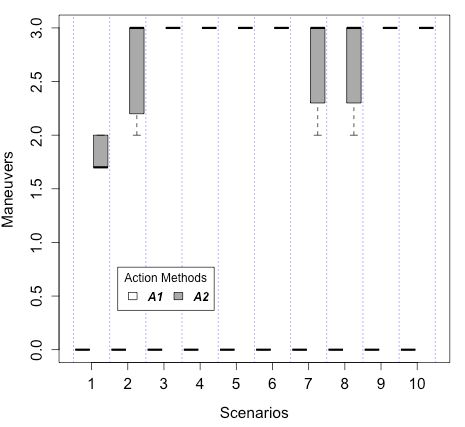
\includegraphics[width=0.95\linewidth]{img/graphs/Boxplot_M2.png}
%   \captionof{figure}{Total of maneuverings(M2)}
%   \label{fig:m2}
% \end{minipage}
% \end{figure}

Notice in Figure~\ref{fig:m3} a significant difference between the system total time in operation of the action methods, i.e., timeliness (M2). The A2 method allowed the system to keep running for a longer time even in scenarios with more events that cause context changes. Figure~\ref{fig:m5} shows that the capacity of the C2 system to solve tasks, under the effect of changes in the context that alter its functioning, is more significant in A2 method.
All C2 Approach changes required by the loss of 60\% of the members and reduction of quality in all sensors onboard caused by the context change events make scenario 3 to show similar results in both action methods (A1 and A2). Scenarios with more context change events presented minor results due to loss of system resources, i.e., members, sensors and autonomy.

% \begin{figure}
% \centering
% \begin{minipage}{.5\textwidth}
%   \centering
%   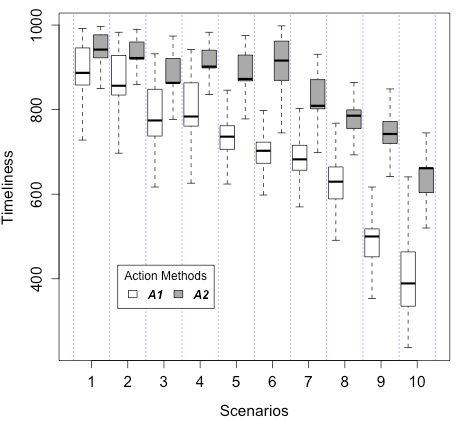
\includegraphics[width=0.95\linewidth]{img/graphs/Boxplot_M3.png}
%   \captionof{figure}{Total operation time(M3)}
%   \label{fig:m3}
% \end{minipage}%
% \begin{minipage}{.5\textwidth}
%   \centering
%   %  \includegraphics[width=0.95\linewidth]{img/graphs/Result_M4.png}
%   \includegraphics[width=0.95\linewidth]{img/graphs/Boxplot_M4.png}
%   \captionof{figure}{Resilience(M4)}
%   \label{fig:m4}
% \end{minipage}
% \end{figure}


% \begin{figure}
% \centering
% \begin{minipage}{.5\textwidth}
%   \centering
%   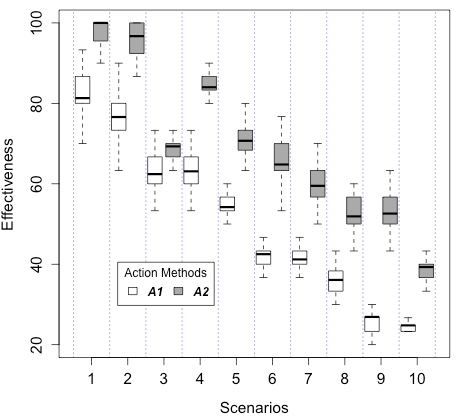
\includegraphics[width=0.95\linewidth]{img/graphs/Boxplot_M5.png}
%   \captionof{figure}{Completed tasks(M5)}
%   \label{fig:m5}
% \end{minipage}%
% \begin{minipage}{.5\textwidth}
%   \centering
%   \includegraphics[width=0.95\linewidth]{img/graphs/Boxplot_M6.png}
%   \captionof{figure}{Total reward(M6)}
%   \label{fig:m6}
% \end{minipage}
% \end{figure}


With a Shapiro-Wilk test~\citep{stat001} a \textit{p-value} less than 0.05 was obtained, thus indicating a non-normal distribution. Based on this, an Mann-Whitney U Test described in ~\cite{stat002} was applied, i.e., Wilcoxon-test in R, to check differences among the samples of each action method applied, i.e., A1 and A2. According to the number and value of samples, the statistical analysis confirmed the difference between all results from A1 and A2 methods, collected in all scenarios tested, including Scenario 3.

The \emph{null hypothesis $H_0$} in Table~\ref{table:hyp} can be refuted since the non-parametric statistical test demonstrated that the results of the metrics defined in GQM are different for the treatments applied to the action method. Even for the scenario 3, the \textit{p-value} was 0.02865 and indicates that the two samples compared, i.e., A1 and A2 results, are statistically different. Based on this, the alternative hypothesis is valid, confirming that the proposed method A2, able to perform C2 Approach changes, presented a significant result in face of context changes simulated.

In addition, it is possible to identify, through the timeliness metric (M3), that more time consumed indicates a capacity to keep running under context perturbations and more resilience of the system to keep running even under such context changes. This characteristic is more present in A2 method due to the proposal tries to adapt itself to deal with these context changes and to keep running. Since removing members through the \emph{memberFailure} event does not allow the system for a reconfiguration due to the member loss, requiring a task reallocation or even a C2 Approach change, it explains the drop shown in scenario 3 of action method A2 to the M3 metric. In turn, \emph{sensorFailure} and \emph{envChange} enable the attempt to reconfigure the member or adjust the C2 Approach in order to search for an optimal allocation of pending tasks, giving to A2 an advantage in all other scenarios. In general, the following empirical findings can be listed:

\begin{itemize}
     \item \textbf{C2 Maneuver Agility}: Based on the obtained results, it is possible to observe a considerable difference in the values obtained with the system running the action method A1, and the system with the capability of C2 Approach change, i.e., with the proposal action method A2. The choice of C2 Approach and how the C2 Approach space is explored comes up against limitations of the entities communication structure, as well as the cost for performing such maneuvers, i.e., time spent and entities' autonomy reduction. Some scenarios required more time to perform the maneuverings, e.g., scenarios 3 to 6, which operated for longer, but could not increase the effectiveness level due to time spent to proceed the C2 Approach changing.
\end{itemize}

 

